\chapter{Baggrund}
\section{Hjertet \& Kredsløb}
Hjertet, \textit{cor}, er en hul muskel, der har til opgave at pumpe blodet rundt til hele kroppen. Hjertet består af i alt fire kamre, som det kan ses på figur 3.1 nedenfor. To forkamre, atrier, og to hjertekamre, ventrikler. Atrierne fungere primært som reservoir for blod, mens ventriklerne fungerer som den effektive pumpe.\\

\begin{figure}[htb]
	\centering
	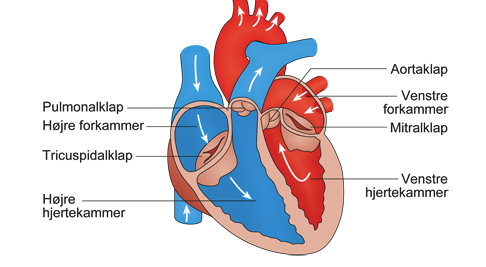
\includegraphics[width=1\textwidth]{Figurer/Fysio/Hjertet}
	\caption{Hjerte med forklarende pile \protect\footnotemark} 
\end{figure}
\footnotetext{http://www.hjertelunge.dk/hjertesygdomme/hjerte\_og\_kredsloeb/hjertet/}

Hjertekamrene og forkamrene er adskilt fra hinanden af anulus fibrosus, som er en plade af bindevæv. Anulus fibrosus består af fire bindevævsringe, der er forbundet med hinanden. To af disse udgør åbningerne mellem atrierne og ventriklerne. De to sidste danner åbningerne mellem højre hjertekammer og lungepulsåren og venstre ventrikel og hovedpulsåren. Ved alle bindevævsringene er der klapper, der fungere som ventiler.\\ 
AV-klapperne sidder mellem atrierne og ventriklerne. Klappen mellem højre atrium og ventrikel kaldes tricuspidalklap, mens klappen mellem venstre atrium og ventrikel kaldes mitralklap, se figur 3.1. Aortaklappen er placeret ved afgangen af hovedpulsåren og pulmonalklappen ved afgangen af lungepulsåren. Klapperne fungere således, at blodet kun kan løbe én vej gennem dem. Åbningen samt lukningen af disse er en passiv proces, som bestemmes af forskelle i væsketrykket på de to sider af klapperne.\\ 

\begin{figure}[htb]
	\centering
	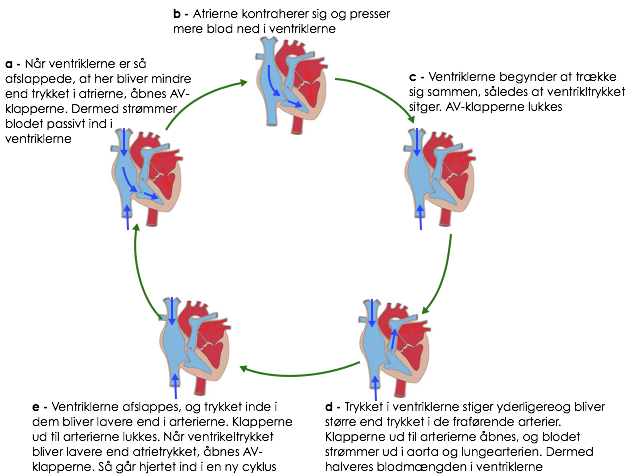
\includegraphics[width=1\textwidth]{Figurer/Fysio/Cyklus}
	\caption{De forskellige faser i hjertets cyklus \protect\footnotemark}
\end{figure}
\footnotetext{Billede fra "Menneskets anatomi og fysiologi" s. 273 figur 9.6}

Hjertets cyklus, som er illustreret ved figur 3.2, inddeles i to hovedfaser. Den første kaldes diastolen. I diastolen er ventriklerne afslappede og fyldes med blod. Det vil sige, at trykket i ventriklerne bliver lavere end trykket i atrierne, således at AV-klapperne åbnes, og blodet begynder at strømme ind i ventriklerne. Under hele diastolen er aortaklappen lukket. Den anden fase kaldes systolen. I systolen kontraherer ventriklerne sig. Trykket i ventriklerne overstiger trykket i atrierne således, at AV-klapperne lukkes, så tilbagestrømning af blod til atrierne forhindres. Når ventriklerne har kontraheret sig så meget, at trykket i ventriklerne overstiger trykket i hovedpulsåren samt i lungepulsåren, åbnes aortaklappen og pulmonalklappen, og blodet strømmer ud i hovedpulsåren og lungepulsåren. Ventriklernes tryk falder igen til under atriernes tryk, hvilket påvirker, at AV-klapperne åbnes igen og hjertets cyklus starter forfra.\\
\section{Blodtryk}
\section{Hypertension}
Hypertension defineres ud fra vedtagne blodtryksgrænser. De nuværende blodtryksgrænser ligger på et systolisk tryk over 140mmHg og/eller diastolisk tryk på over 90mmHg. Disse grænser gælder uanset patientens alder. Grænseværdierne er dog kun et udgangspunkt for der kan godt opstå hypertension hos en person med forvejen for lavt tryk og i dette tilfælde vil grænseværdierne ikke nå op på værdien for definitionen af hypertension.\\
Hypertension medfører betydelig øget risiko for kardiovaskulære sygdomme som oftest er apopleksi og iskæmisk hjertesygdom. Herudover kan hypertension medfører påvirkning af nyrene.
\footnote{https://www.sundhed.dk/sundhedsfaglig/laegehaandbogen/hjerte-kar/tilstande-og-sygdomme/oevrige-sygdomme/hypertension/} 

\section{Hypotension}
\section{Hæmodynamik}

